% !TEX TS-program = pdflatex
% !TEX encoding = UTF-8 Unicode

% This file is a template using the "beamer" package to create slides for a talk or presentation
% - Talk at a conference/colloquium.
% - Talk length is about 20min.
% - Style is ornate.

% MODIFIED by Jonathan Kew, 2008-07-06
% The header comments and encoding in this file were modified for inclusion with TeXworks.
% The content is otherwise unchanged from the original distributed with the beamer package.


\documentclass{beamer}

% Copyright 2004 by Till Tantau <tantau@users.sourceforge.net>.
%
% In principle, this file can be redistributed and/or modified under
% the terms of the GNU Public License, version 2.
%
% However, this file is supposed to be a template to be modified
% for your own needs. For this reason, if you use this file as a
% template and not specifically distribute it as part of a another
% package/program, I grant the extra permission to freely copy and
% modify this file as you see fit and even to delete this copyright
% notice. 

\usepackage[english,polish]{babel}

\mode<presentation>
{
  \usetheme{Warsaw}
  % or ...

  \setbeamercovered{transparent}
  % or whatever (possibly just delete it)
}


% or whatever

\usepackage[utf8]{inputenc}
% or whatever

\usepackage{times}
\usepackage[T1]{fontenc}
% Or whatever. Note that the encoding and the font should match. If T1
% does not look nice, try deleting the line with the fontenc.
\usepackage{booktabs} % for much better looking tables
\usepackage{array} % for better arrays (eg matrices) in maths
\usepackage{paralist} % very flexible & customisable lists (eg. enumerate/itemize, etc.)
\usepackage{verbatim} % adds environment for commenting out blocks of text & for better verbatim
\usepackage{subfig} % make it possible to include more than one captioned figure/table in a single float
\usepackage{multicol}
\usepackage{amsmath}
\usepackage{amssymb}
\usepackage{bm}
\usepackage{svg}
\usepackage{amsthm}
\usepackage{ bbold }
\usepackage{eufrak}
\usepackage[titletoc,title]{appendix}
\newcommand{\Mats}[1]{\mathcal{L}(#1)}
\newcommand{\Hx}[1]{\mathcal{H}^{#1}}
\newcommand{\LHx}[1]{\Mats{\Hx{#1}}}
\newcommand{\HAi}{\Hx{A_1}}
\newcommand{\LHAi}{\Mats{\HAi}}
\newcommand{\MXi}[3]{\mathcal{M}^{#1}_{#2}(#3)}
\newcommand{\MXin}[2]{\mathcal{M}^{#1}_{#2}}
\newcommand{\MAin}[0]{\MXin{A}{i}}
\newcommand{\MAi}[1]{\MXi{A}{i}{#1}}
\newcommand{\MAir}{\MAi{\rho}}
\newcommand{\Idx}[1]{\mathbb{1}^{#1}}
\newcommand{\Tr}[1]{\Trs(#1)}
\newcommand{\Pro}[1]{\Pr(#1)}
\newcommand{\Prt}[2]{\Pr(#1, #2)}
\newcommand{\Ket}[1]{|#1\rangle}
\newcommand{\Bra}[1]{\langle#1|}
\newcommand{\BBra}[1]{\langle\langle#1|}
\newcommand{\KKet}[1]{|#1\rangle\rangle}
\newcommand{\Braket}[1]{\langle#1\rangle}
\newcommand{\CP}{\textit{completely positive}}
\newcommand{\TP}{\textit{trace preserving}}
\newcommand{\CPTP}{\textit{completely posite trace preserving}}
\newcommand{\WAll}{W^{A_1A_2B_1B_2}}
\newcommand{\MA}{M^{A_1A_2}}
\newcommand{\MB}{M^{B_1B_2}}
\newcommand{\mai}[1]{\MA_{#1}}
\newcommand{\mbi}[1]{\MB_{#1}}
\newcommand{\KP}{\Ket{\psi}}
\newcommand{\BP}{\Bra{\psi}}
\newcommand{\X}{\mathbb{X}}
\newcommand{\Y}{\mathbb{Y}}
\newcommand{\Z}{\mathbb{Z}}
\newcommand{\I}{\mathbb{1}}
\newcommand{\IO}{\mathbb{1}^\circ}
\newcommand{\MCJ}{\mathfrak{C}}
\newcommand{\LV}{L_V}
\newcommand{\LPV}{{L^\perp_V}}
\DeclareMathOperator{\Trs}{Tr}
\DeclareMathOperator{\Rank}{rank}
\title[] % (optional, use only with long paper titles)
{Przyczynowe więzy na strukturę korelacji w formalizmie
kwantowym}


\author[Piotr Krasuń]
{}
\institute[Politechnika Gdańska] % (optional, but mostly needed)
{
Politechnika Gdańska \\
  Wydział Fizyki Technicznej i Matematyki Stosowanej
}
% - Use the \inst command only if there are several affiliations.
% - Keep it simple, no one is interested in your street address.


% If you have a file called "university-logo-filename.xxx", where xxx
% is a graphic format that can be processed by latex or pdflatex,
% resp., then you can add a logo as follows:

% \pgfdeclareimage[height=0.5cm]{university-logo}{university-logo-filename}
% \logo{\pgfuseimage{university-logo}}



% Delete this, if you do not want the table of contents to pop up at
% the beginning of each subsection:
\AtBeginSubsection[]
{
  \begin{frame}<beamer>{Zarys}
    \tableofcontents[currentsection,currentsubsection]
  \end{frame}
}


% If you wish to uncover everything in a step-wise fashion, uncomment
% the following command: 

%\beamerdefaultoverlayspecification{<+->}


\begin{document}

\begin{frame}
  \titlepage
\end{frame}

\begin{frame}{Zarys}
  \tableofcontents
  % You might wish to add the option [pausesections]
\end{frame}


% Structuring a talk is a difficult task and the following structure
% may not be suitable. Here are some rules that apply for this
% solution: 

% - Exactly two or three sections (other than the summary).
% - At *most* three subsections per section.
% - Talk about 30s to 2min per frame. So there should be between about
%   15 and 30 frames, all told.

% - A conference audience is likely to know very little of what you
%   are going to talk about. So *simplify*!
% - In a 20min talk, getting the main ideas across is hard
%   enough. Leave out details, even if it means being less precise than
%   you think necessary.
% - If you omit details that are vital to the proof/implementation,
%   just say so once. Everybody will be happy with that.

\section{Porządek przyczynowy}

\subsection{Klasyczny porządek przyczynowy}

\begin{frame}{Wydarzenia uporządkowane przyczynowo $t_1$.}
\centering
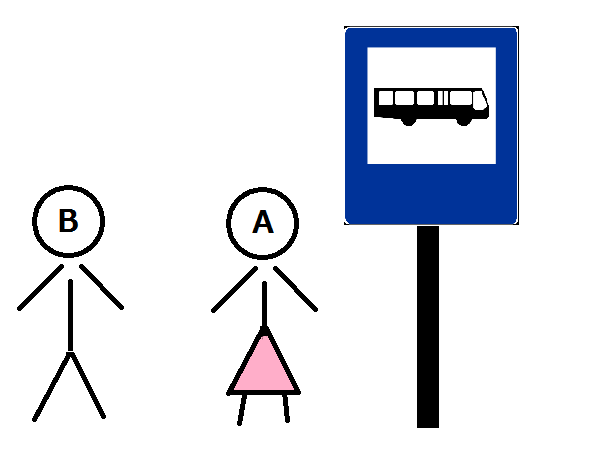
\includegraphics[width=0.8\textwidth]{obrazki/pAB}
\end{frame}

\begin{frame}{Wydarzenia uporządkowane przyczynowo $t_2$.}
\centering
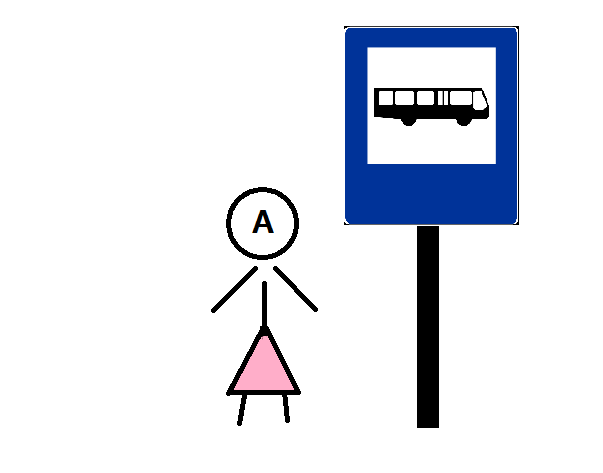
\includegraphics[width=0.8\textwidth]{obrazki/pA}
\end{frame}

\begin{frame}{Wydarzenia uporządkowane przyczynowo $t_2$.}
\centering
\begin{tabular}{|c|c|}
\hline\\
$p$ & $1-p$ \\
\hline
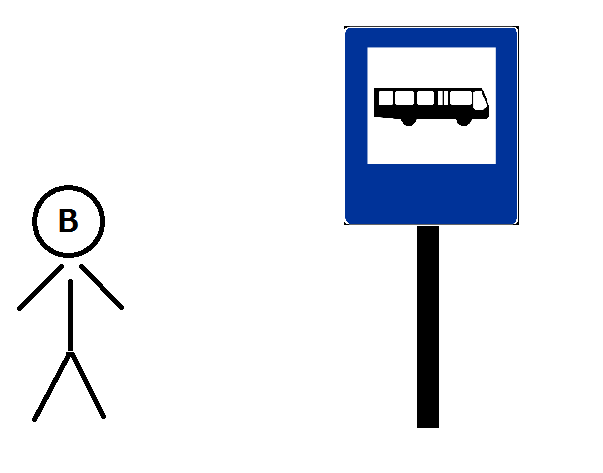
\includegraphics[width=0.4\textwidth]{obrazki/pB} & 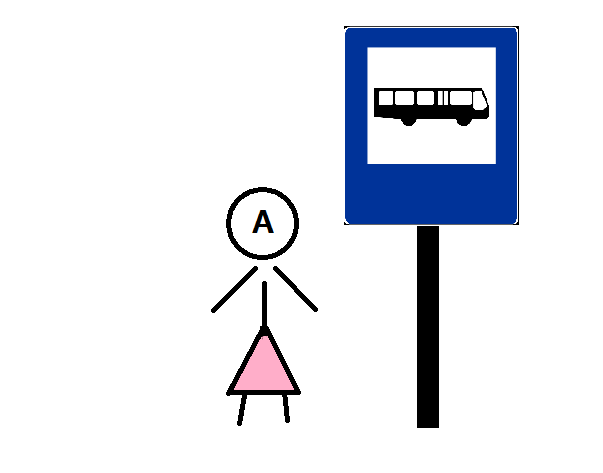
\includegraphics[width=0.4\textwidth]{obrazki/pA}\\
\hline
\end{tabular}
\end{frame}

\begin{frame}{Wydarzenia uporządkowane przyczynowo $t_3$.}
\centering
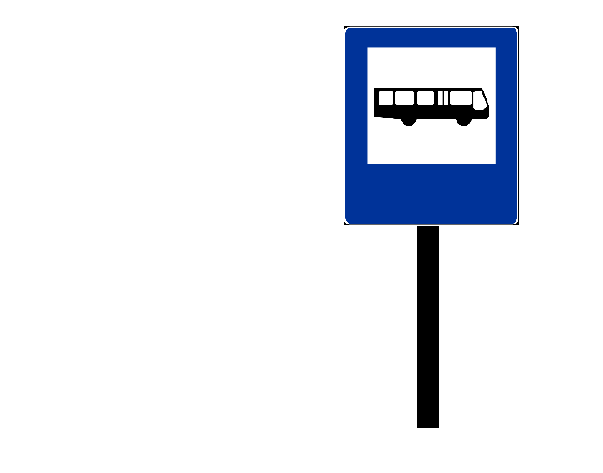
\includegraphics[width=0.8\textwidth]{obrazki/p}
\end{frame}

\subsection{Brak porządku przyczynowego}

\begin{frame}{Porządek generowany przez macierze procesu $t_P$.}
\centering
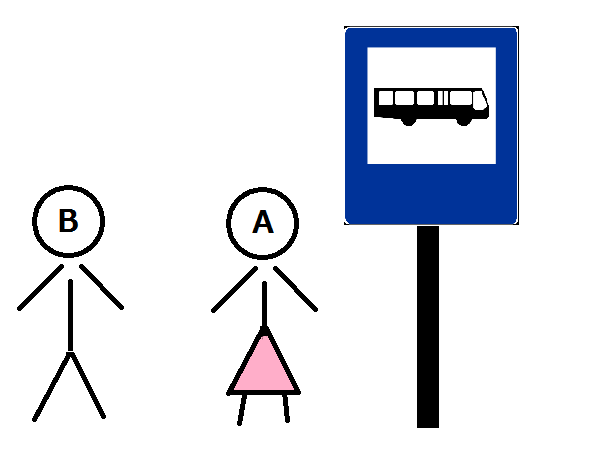
\includegraphics[width=0.8\textwidth]{obrazki/pAB}
\end{frame}

\begin{frame}{Porządek generowany przez macierze procesu $t_W$.}
\centering
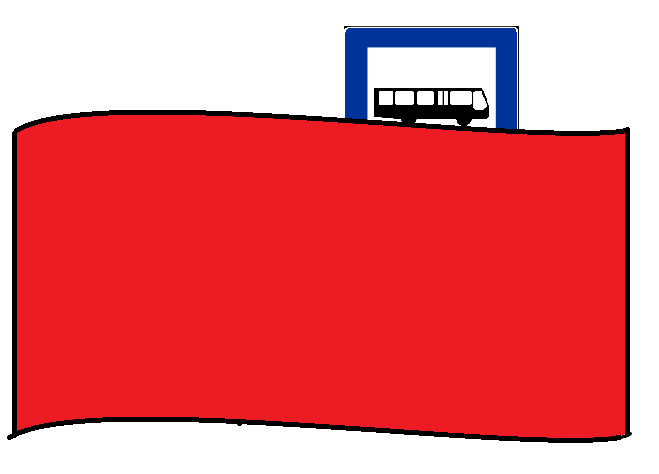
\includegraphics[width=0.8\textwidth]{obrazki/pW}
\end{frame}

\begin{frame}{Porządek generowany przez macierze procesu $t_F$.}
\centering
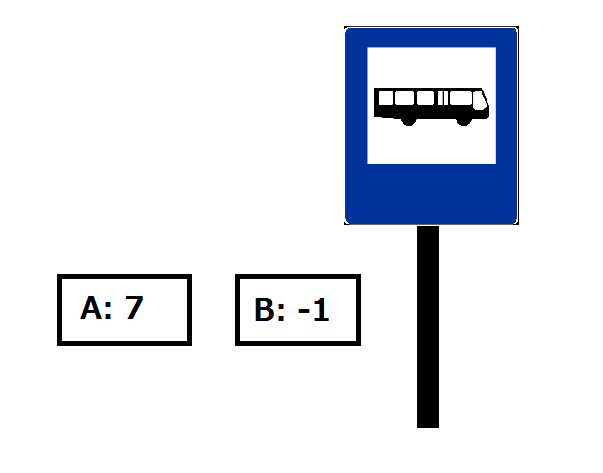
\includegraphics[width=0.8\textwidth]{obrazki/pF}
\end{frame}

\begin{frame}{Porządek generowany przez macierze procesu $t_F$.}
\centering
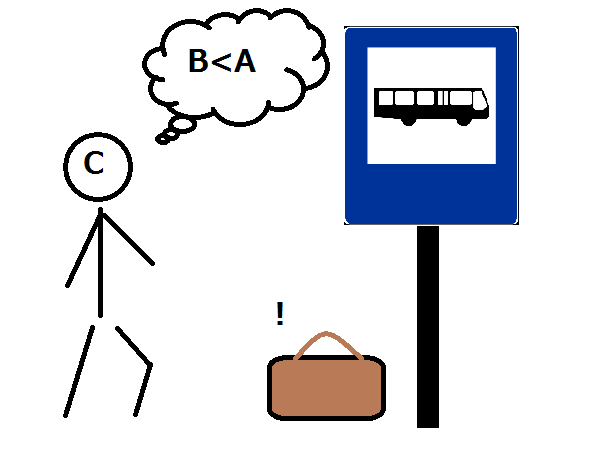
\includegraphics[width=0.8\textwidth]{obrazki/pC}
\end{frame}

\section{Macierz procesu}
\subsection{Macierz procesu}
\begin{frame}{Izomorfizm CJ}
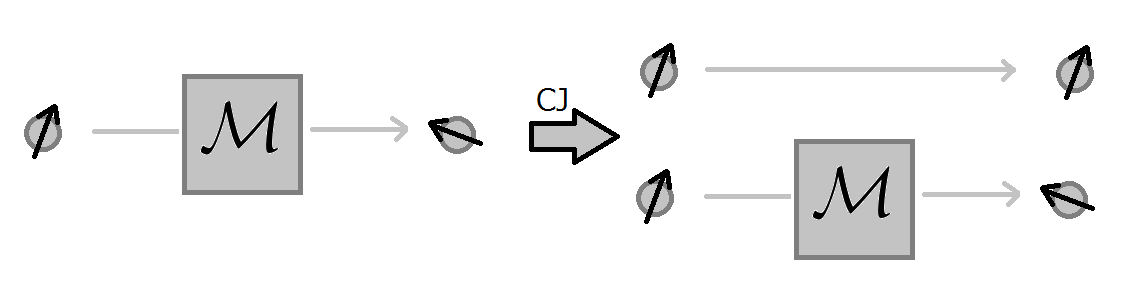
\includegraphics[width=0.8\textwidth]{obrazki/cj_new}
\begin{gather}
\mathfrak{C}(\mathcal{M_i}) = \left[\sum_{ij} \Ket{i}\Bra{i} \otimes \mathcal{M_i}\left(\Ket{i}\Bra{j}\right)\right]^T\\
\KKet{A} = \sum_i \left( \Ket{i}\otimes A\Ket{i}\right)
\end{gather}
\end{frame}

\begin{frame}{Warunki na macierz procesu}
\centering
\begin{gather}
W  \in \Mats{\Hx{A_1} \otimes \Hx{A_2} \otimes \Hx{B_1} \otimes \Hx{B_2}}\\
W \geq 0 \\
\Trs W=d_{A_2B_2}\\
\Pr(i,j) = \Trs\left[ W \left( M_i \otimes M_j\right)\right]
\end{gather}
\end{frame}

\subsection{Klasyczne elementy}
\begin{frame}{Stany}
\centering
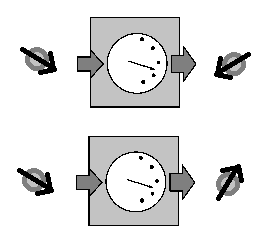
\includegraphics[width=0.4\textwidth]{obrazki/states_new}\\
\begin{equation}
W = \rho^{A_1B_1} \otimes \I^{A_2B_2}
\end{equation}
\end{frame}

\begin{frame}{Kanały}
\centering
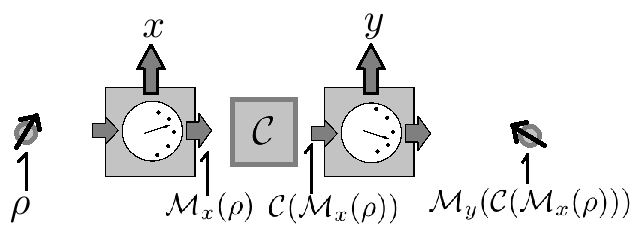
\includegraphics[width=0.8\textwidth]{obrazki/channel_new}\\
\begin{equation}
W = \rho^{A_1} \otimes C^{A_2B_1} \otimes \I^{B_2}
\end{equation}
\end{frame}

\begin{frame}{Kanały z pamięcią}
\centering
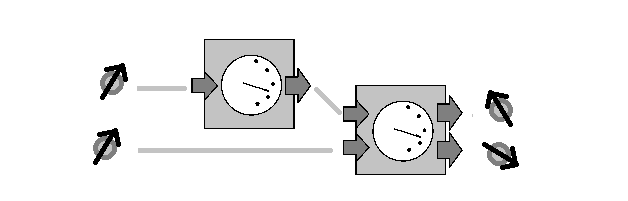
\includegraphics[width=0.8\textwidth]{obrazki/memory_new}\\
Wyrazy typu $A_1A_2B_1$, $B_1B_2A_1$.
\end{frame}

\subsection{Kwantowy przełącznik}
\begin{frame}{Ważny przykład}
\centering
\begin{figure}
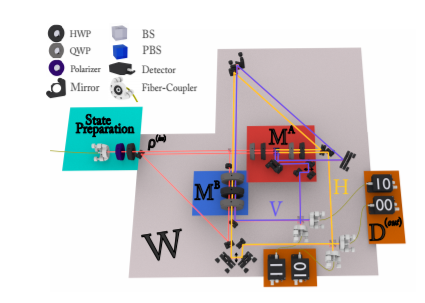
\includegraphics[width=0.3\textwidth]{obrazki/qs}
\caption{Ilustracja kwantowego przełącznik, źródło: \cite{experiment}}
\end{figure}
\begin{equation}
\begin{split}
\Ket{w} =& \Ket{\psi}^{A_1}\KKet{\I}^{A_2B_1}\KKet{B_2C_{1t}}\Ket{0}^{C_c}\\
&+ \Ket{\psi}^{B_1}\KKet{\I}^{B_2A_1}\KKet{\I}^{A_2C_{1t}}\Ket{1}^{C_c}
\end{split}
\end{equation}
\end{frame}
\subsection{Gry przyczynowe}
\begin{frame}{Łamanie nierówności przyczynowych}
\centering
\begin{equation}
\frac{1}{4}\left[
\I\I\I\I + \frac{1}{\sqrt{2}}(\I\Z\Z\I + \Z\I\X\Z)
\right]
\end{equation}
\begin{equation}
\Pr{}_{sukces} \geq \frac{3}{4}
\end{equation}
\end{frame}
\subsection{Świadek przyczynowości}
\begin{frame}{Świadek przyczynowości}
\centering
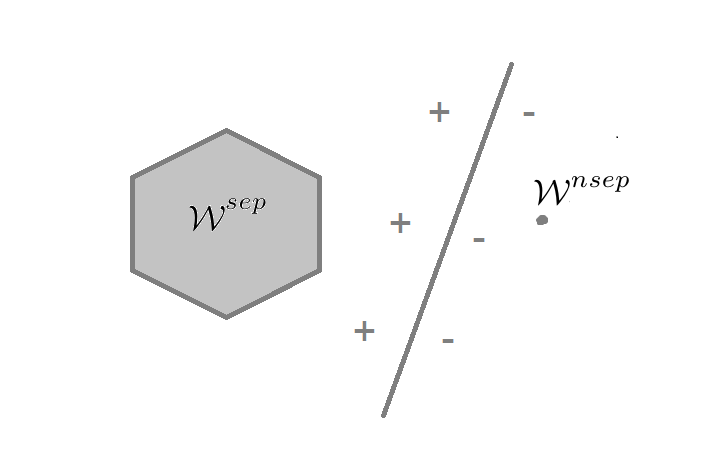
\includegraphics[width=0.45\textwidth]{obrazki/hip}
\begin{gather}
\Trs\left[ W^{sep}S\right] \geq 0 \\
\min \Trs \left[ WS \right]\\
\text{tak, aby } S \in \mathcal{S_V},~ \frac{\I}{d_O} - S \in \mathcal{W^*_V},
\end{gather}
\end{frame}

\begin{frame}[allowframebreaks]
  
\bibliographystyle{plain}
\bibliography{bibliografia}
\end{frame}

\end{document}


